\begin{slikaDesno}{fig/exp_osc.pdf}
\PID У колу са слике познато је 
$R = 1\unit{k\Upomega}$, $C=1\unit{\upmu F}$ и 
напон напајања $V_{\rm CC} = 5\unit{V}$.
Систем „К“ управља идеалним прекидачем П 
на основу напона $v_{C}$. Прекидач П је иначе 
отворен, уколико напон $v_{\rm C}$ достигне вредност 
$mV_{\rm CC}$, где је $0 \leq m \leq 1$ позната 
константа, контролни систем „K“ тренутно и 
\textit{краткотрајно} затвара прекидач. У почетном 
тренутку је $v_{\rm C}(0) = 0$. 
\begin{enumerate}[label=(\alph*)]
\item Одредити  напон 
на кондензатору у зависности од времена, и нацртати његов временски 
дијаграм за $m = \dfrac{1}{2}$; и
\item одредити спектралне коефицијенте 
тог напона на његовом основном периоду у устаљеном 
сложенопериодичном режиму. 
\end{enumerate}
\end{slikaDesno} \\


\underline{\sc Решење:} 

(а) Кондензатор се пуни струјом из извора напајања, напона $V_{\rm CC}$,  
преко отпорника отпорности $R$. Израз за напон кондензатора у том случају је 
\begin{equation}
v_{C}(t) = V_{\rm CC} \left(
    1 - \ee^{-t/\uptau} 
\right), \label{eq:\ID.vc}
\end{equation} где је $\uptau = RC$ временска константа посматраног система првог реда. Пуњење кондензатора траје
све док је $v_C(t) < m V_{\rm CC}$. У граничном случају је, 
$v_C(T) = m V_{\rm CC}$, одатле се може одредити тренутак $T$ када се први пут затвара прекидач. 
Има се резултат
\begin{equation}
    \cancel {V_{\rm CC}} \left(
    1 - \ee^{-T/\uptau} \right) = m \cancel{V_{\rm CC}}
    \Rightarrow \ln(1 - m) = -\dfrac{T}{\uptau} \Rightarrow 
    T = \uptau \ln \left( \dfrac{1}{1 - m} \right).
\end{equation}

Након затварања прекидача је $v_{C}(T^+) = 0$, односно, краткотрајно затварање идеалног прекидача 
у потпуности растерећује кондензатор, након чега се пређашњи процес понавља. 
Односно, процес описан изразом \eqref{eq:\ID.vc} у домену 
$\DS 0 < t < T = \uptau \ln \left( \dfrac{1}{1 - m} \right)$, представља основни период напона
на кондензатору. 

Уколико се замене дате вредности има се да је временска константа 
$\uptau = 1\unit{ms}$, и да је $T = \uptau \ln 2 \approx 0,69 \unit{ms}$. 
Тражени временски дијаграм приказан је на слици \ref{fig:\ID.2}. На истом дијаграму, испрекиданом
линијом приказан је и продужетак дијаграма првобитног пуњења кондензатора -- који илуструје да би 
у недостатку прекидача тај напон асимптотски растао до напона напајања. 

\begin{figure}[ht!]
    \centering
    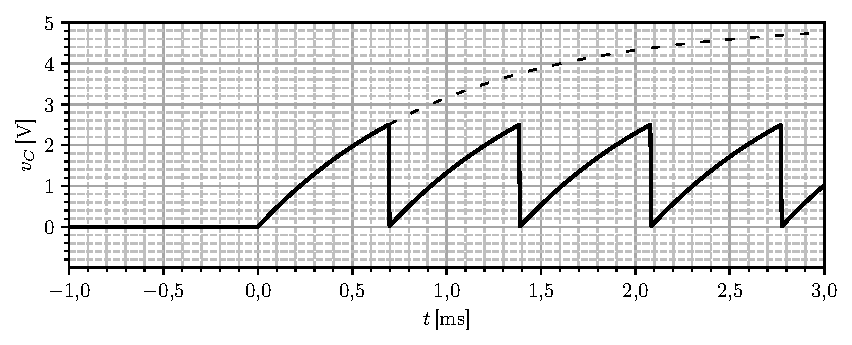
\includegraphics[scale=1]{fig/exp_osc_plot.pdf}
    \caption{Пример временског дијаграма за $m = \dfrac{1}{2}$, $V_{\rm CC} = 5\unit{V}$. }
    \label{fig:\ID.2}
\end{figure} 

(б) Развој у Фуријеов ред може се поједноставити применом особине суперпозиције
$\FS{ v_C(t) } = 
\FS{ V_{\rm CC} \left(
    1 - \ee^{-t/\uptau} \right) } 
= V_{\rm CC} \left(
    \FS{1}
    -
    \FS{
    \ee^{-t/\uptau}    
    }
\right) 
= V_{\rm CC} \left(
\updelta[k] 
-
\FS{
    \ee^{-t/\uptau}    
    }
\right).
$ 
Развој преосталог члана, експоненцијалног сигнала, у Фуријеов ред може се обавити по 
дефиницији\footnote{
    Развој у Фуријеов ред по дефиницији 
    $\DS\FS{x(t)} = \dfrac{1}{T}\int_{\langle T \rangle} x(t) \ee^{-\jj k \upomega_{\rm F} t} \de t$.
}, за $\upomega_{\rm F} = \upomega_0$
решавањем интеграла\footnote{Користи се интеграл 
    $\int e^{kx} \de x = e^{kx}/k + C$.
} 
\begin{equation}
    \FS{
    \ee^{-t/\uptau}    
    }
    = \dfrac{1}{T}\int_0^T 
    \ee^{-t/\uptau} \ee^{-\jj k \upomega_0 t} \,\de t
    =
    \dfrac{1}{T}\int_0^T 
    \ee^{-\left( \jj k\upomega_0  +  1/\uptau \right) t } \,\de t
    = 
    -\dfrac{
        \ee^{-\left( \jj k \cancelto{2\uppi}{\upomega_0 T}  +  T/\uptau \right) }
        - 1
    }{ \jj k \cancelto{ 2\uppi }{\upomega_0 T}  +  T/\uptau }.
\end{equation}
Приметимо да је 
$
\ee^{ -\left( \jj 2\uppi k  +  T/\uptau \right)} 
= \cancelto{1}{\ee^{\jj 2\uppi k}} + {1-m} = 2 - m$, па се коначно има: 
$
\FS{
    \ee^{-t/\uptau}    
    } =
    \dfrac{m - 1}{
        \jj 2\uppi k - \ln\left( 1 - m \right)
    }.
$ Коначно, добија се да је развој траженог сигнала у Фуријеов ред дат изразом
$V_C[k] = 
V_{\rm CC} \left(
    \updelta[k] 
        - 
        \dfrac{m - 1}{
            \jj 2\uppi k - \ln\left( 1 - m \right)
        }
\right)$. \\

Представљени систем представља једно принципско решење за пројектовање осцилатора 
(тзв. \textit{релаксациони осцилатор}). Променом границе укључења контролера који практично
ресетује напон кондензатора, односно променом 
параметра $m$,
мења се учестаност осциловања. Систем за контролу „К“ може се реализовати са једним операционим
појачавачем који се понаша као компаратор, док је прекидач могуће реализовати као нпр. MOS 
транзистор. 
